\documentclass[12pt,a4paper]{report}
\usepackage[a4paper, top=0.98in, bottom=0.98in, left=1.85in, right=0.79in]{geometry}
\usepackage{graphicx}
\usepackage{fancyhdr}  % For custom headers and footers
\usepackage{titlesec}  % For customizing title formats
\usepackage{setspace}  % For line spacing
\usepackage[absolute,overlay]{textpos}
\usepackage{tikz}
\usetikzlibrary{positioning}
\usepackage{booktabs} % For better-looking tables
\usepackage{amsmath} 
\usepackage{url}
\usepackage{xcolor} % for text coloring
\usepackage{listings}


% Set up spacing
\onehalfspacing

% Format chapter titles
\titleformat{\chapter}[display]
  {\normalfont\Huge\bfseries}{\chaptertitlename\ \thechapter}{20pt}{\Huge}
\titlespacing*{\chapter}{0pt}{180pt}{18pt}


% let it number up to subsubsection
\setcounter{secnumdepth}{3}

% Make sure chapter titles appear correctly in the header
\renewcommand{\chaptermark}[1]{\markboth{#1}{}}

\begin{document}

% Cover page
\newcommand{\titlefont}{\fontfamily{ptm}\fontsize{18}{22}\selectfont\bfseries}

\begin{titlepage}
    
    \begin{tikzpicture}[overlay, remember picture]
        % Vertical line
        \draw[thick] (current page.south west) ++(1.7in, 0) -- ++(0, \paperheight - 2.1in); 
        
    \end{tikzpicture}

   \begin{textblock*}{1cm}(1.0in, 5in)  % Adjust position as needed
   	\centering
   	\rotatebox{-90}{
   		\begin{minipage}{14cm}  % Adjust width as needed
   			\centering
   			Mosaned | Navigation and Guidance System for Indoor Environments for Blind and Visually Impaired Individuals 
   		\end{minipage}
   	}
   \end{textblock*}
   
    \vspace*{1.2in}
    \centering
    
     % Uni coordinates for the image placement
    \begin{textblock*}{1.04in}(0.7in,3.3in)
    
\includegraphics[width=0.576in,height=0.7488in]{assets/uni.png}
    \end{textblock*}
    
    % Uni coordinates for the image placement
    \begin{textblock*}{1.04in}(2.2in,1in)
    
\includegraphics[width=0.8in,height=1.04in]{assets/uni.png}
    \end{textblock*}

    % Dep. coordinates for the image placement
    \begin{textblock*}{1.04in}(6in,1.1in)
    
\includegraphics[width=1.4in,height=1.04in]{assets/dep.png}
    \end{textblock*}

    {\titlefont \textbf{Taibah University}}\\
    {\titlefont \textbf{College of Computer Science Engineering}}\\
    {\titlefont \textbf{Computer Engineering Department}}\\
    
    \vspace{1.8cm}
    
    {\titlefont \textbf{Mosaned | Navigation and Guidance System for Indoor Environments for Blind and Visually Impaired Individuals}}
    
    \vspace{1.8cm}

    {\titlefont \fontsize{14}{16} \textbf{A Project Submitted in partial fulfilment of the requirements for the Bachelor Degree in Computer Engineering}}
    \vspace{1.8cm}
    
    \vspace{1.2cm}
    
    \begin{minipage}{\textwidth}
    	\centering
    	{\titlefont \textbf{Submitted By}}\\
    	\vspace{1cm}
    	
    	\begin{tabular}{@{}l@{\hskip 4cm}r@{}}
    		{\titlefont \textbf{Mohammed Alharbi}} & {\titlefont \textbf{4200174}} \\
    		{\titlefont \textbf{Firas Alsadeq}} & {\titlefont \textbf{4200625}} \\
    		{\titlefont \textbf{Mousa Alenzi}} & {\titlefont \textbf{4106574}} \\
    	\end{tabular}
    \end{minipage}
    
    \vspace{1.8cm}

    {\fontfamily{ptm}\selectfont\fontsize{14}{16}\normalfont
    \textbf{Project Advisor}\\
    Dr. Moteb Alghamdi
    }
    
    \vspace{2cm}

    {\fontfamily{ptm}\selectfont\fontsize{14}{16}\normalfont
    \textless 2024-2025\textgreater-\textless 1st Semester\textgreater
    }

\end{titlepage}


\pagenumbering{roman}



\newpage
\thispagestyle{plain}
\setcounter{page}{1}
\renewcommand{\thepage}{\roman{page}}

\begin{center}
    \Large\textbf{ABSTRACT}
\end{center}
\vspace{6pt}


Visually impaired and blind individuals might face difficult challenges when navigating through indoor environments, especially if they where not familiar with them. Indoor environments can be very unpredictable and filled with obstacles, and they are rich of important visual information which only designed for eyes consumption. These difficulties rise the need of these individuals to assistants and guiders whether by asking strangers, or by taking companions. But
these solutions will lead to decreasing the independence of these individuals. We are trying to offer a solution in this project, a wearable and easy to use system that guides and assists the users after determining their positions and scanning their surrounding environments using only a camera and smart phone. The proposed system is an integration of three systems: Objects Detection, Localization, and Customizable Guidance System. These components rely on analyzing the images captured by a camera and extracting the important visual information from them. The Objects Detection System can detects the surrounding objects and describe them to the users if they asked to, and informusers about obstacles, and users can ask it to alarm them when they face an object with certain characteristics, such as a main wearing red T-Shirt. The localization system will use the camera to detect artificial landmarks to determine the user’s location. And finally, the Customizable Guidance System reads to user custom information and instructions after entering specific areas. \\
\textcolor{red} {
	- the result obtained\\
	- the significance of the result or finding 
}





\vspace{18pt}
\noindent
\textbf{KEYWORDS:}  Localization; Obstacles Avoidance; Objects Detection, Customization; Guidance; Pose; Calibration
\vspace{3\baselineskip}
\newpage
\thispagestyle{plain}
\setcounter{page}{2}
\renewcommand{\thepage}{\roman{page}}

\begin{center}
    \Large\textbf{ACKNOWLEDGEMENTS}
\end{center}
\vspace{6pt}

The content of this single page is left to the preference of the student.  It is suggested however that the page makes reference to guidance received by the student from his or her supervisor and project Committee members.  Reference should also be made to any financial assistance received to carry out the project.  Any extraordinary assistance received by the student for example in word processing, data collection, data analysis, and so on, should be properly acknowledged.  The acknowledgements should not exceed 250 words.
\color{black}

% Table of Contents
\clearpage
\color{red}
\tableofcontents
\color{black}

\color{red}
\clearpage
\addcontentsline{toc}{chapter}{List of Tables}
\listoftables
\color{black}

\color{red}
\clearpage
\addcontentsline{toc}{chapter}{List of Figures}
\listoffigures
\color{black}

\color{red}
\clearpage
\color{red}

\chapter*{Glossary and List of Abbreviations}

\section*{Glossary}
\begin{description}
  \item[Term 1] Definition of term 1.
  \item[Term 2] Definition of term 2.
\end{description}

\section*{List of Abbreviations}
\begin{description}
  \item[Abbr.] Full form of the abbreviation.
\end{description}

\color{black} % Include glossary and list of abbreviations
\addcontentsline{toc}{chapter}{Glossary and List of Abbreviations} 
\color{black}

% Reset page numbering and start Arabic numbering

\clearpage
\pagenumbering{arabic}
\setcounter{page}{1} % Start Arabic page numbering from 1

% Set up fancyhdr for custom headers
\pagestyle{fancy}
\fancyhf{} % Clear all header and footer fields
\fancyhead[L]{\text{Chapter \thechapter{}} - \small{\leftmark}}

\fancyfoot[C]{\thepage} % Centered page number in the footer
\renewcommand{\headrulewidth}{0.4pt} % Line below the header

\chapter{Introduction}

% ========= BEGIN: CHAPTER-1 ======== %
\newpage
\section{Overview}
\color{red}
This project focuses on using a camera and QR codes for precise localization, allowing the device to determine its exact location. When the camera scans a QR code, it not only identifies where it is but can also trigger additional features like specific instructions or location-based descriptions. This localization system is particularly useful for robots to navigate accurately or for visually impaired people to receive important information about their surroundings.
\color{black}


\section{Motivation}
This project is motivated by the need to enhance the quality of life and autonomy for visually impaired individuals, especially in interior settings where conventional navigation aids such as GPS are inadequate. Visually impaired individuals encounter significant obstacles when navigating intricate indoor environments, which can restrict their mobility and independence. Existing options, such as guide dogs and human aid, although beneficial, may prove inadequate or unworkable in all situations.
The motivation also is to develop a prototype solution utilising commonly accessible technology (such as QR codes and mobile devices) enhances the system's accessibility to a broader audience (Cost and Accessibility). This differs from expensive or complex systems that may require specialized hardware.

\section{Problem Statement}
Navigating indoor environments is challenging for visually impaired individuals, directly affecting their independence and daily activities. While some existing technologies have developed separate algorithms for indoor localization, they are often not integrated into a user-friendly device that individuals can easily use. Moreover, many solutions rely on expensive sensors, increasing the overall cost of the device. Additionally, the majority of current aids do not provide a cohesive approach that combines accurate localization with obstacle detection, and they often lack context-specific, non-visual instructions tailored to the unique needs of visually impaired users. This highlights the urgent need for an affordable, integrated indoor navigation system that enhances mobility and independence in everyday settings.
\section{Project Objectives}

The primary objectives of this project are as follows:

\begin{itemize}
	\item To develop an intuitive and accessible mobile application that enables visually impaired individuals to navigate unfamiliar indoor environments with confidence and ease.
	\item To enhance the independence of visually impaired users by providing a reliable system for localization, obstacle detection, and customizable guidance.
	\item To increase spatial awareness for visually impaired users by offering real-time feedback on their surroundings using accessible technologies like vibration motors and voice guidance.
	\item To design a user-friendly dashboard for building managers, facilitating the integration of the system into buildings by allowing them to manage, configure, and export QR codes effortlessly.
	\item To ensure the system is cost-effective and leverages widely available technologies, making it accessible to a broader audience and promoting widespread adoption.
\end{itemize}

\section{Project Outline}
The remainder of this report is organised as follows: Chapter 2 provides the Background and the related works. Chapter 3 provides the methodology, and Chapter 4  results and discussion. Chapter 5 provides the conclusion and future work.





% ========= BEGIN: CHAPTER-2 ======== %
\chapter{Background}
\newpage
\section{Introduction}


This chapter is organized as follows: Section 2 discusses the role of landmarks in localization, emphasizing artificial landmarks such as QR codes. Section 3 explores the structure, versions, and encoding of QR codes, while Section 4 focuses on QR code-based localization systems. Section 5 covers the Android platform, followed by Section 6, which addresses Google's TalkBack service. Section 7 is about ESP32, followed by sections 8 and 9 which focus on the ultrasonic sensor and the vibration motor respectively. Finally, Section 10 reviews related work in the field.
\section{Landmarks}

Landmarks are essential in navigation, tracking, and mapping, helping to determine positions within an environment. They can be categorized into two types: natural and artificial.

\subsection{Natural Landmarks}

Natural landmarks are features formed by nature or naturally present in an environment, such as mountains, rocks, trees, stairs, or doors. In computer science, they can be used in computer vision algorithms to help determine object locations, create 3D maps, or monitor object states. However, natural landmarks are more difficult to recognize due to their diversity, lack of uniform shapes, and inability to encode data.

\subsection{Artificial Landmarks}

Artificial landmarks, on the other hand, are human-made structures like traffic signs, statues, and QR codes. These landmarks offer several advantages over natural ones in computer vision applications due to their uniformity, ease of recognition, ability to encode data, and customization options. Artificial landmarks are more reliable, precise, and adaptable, making them better suited for controlled environments. Furthermore, many libraries support the encoding, detection, decoding, and tracking of artificial landmarks. Examples include various markers such as QR codes, Aruco markers, and Topotags, which are widely used in different computer science fields. More details on different types of markers can be found in reference \cite{Fiducial2021}.



\section{QR code}
Quick Response (QR) codes are a type of matrix barcode designed for efficient data encoding and rapid scanning. QR Codes first developed in 1994 by Denso Wave, to track automotive parts in manufacturing. but have since become widely used across various applications due to their versatility, simplicity, and capacity to store significant amounts of information compared to traditional barcodes.

\subsection{QR Structure}
QR Codes can be detected and decoded at various angles and distortion levels due to their unique structure. The code consists of black modules (squares) arranged on a white background in a grid pattern, allowing for rapid and error-resistant scanning. All QR Codes have standard structure as shown in Figure \ref{QR_code_structure}. This structure
is made out of the following parts:

\begin{figure}[h] % [h] forces the figure to be placed exactly here in the text
	\centering
	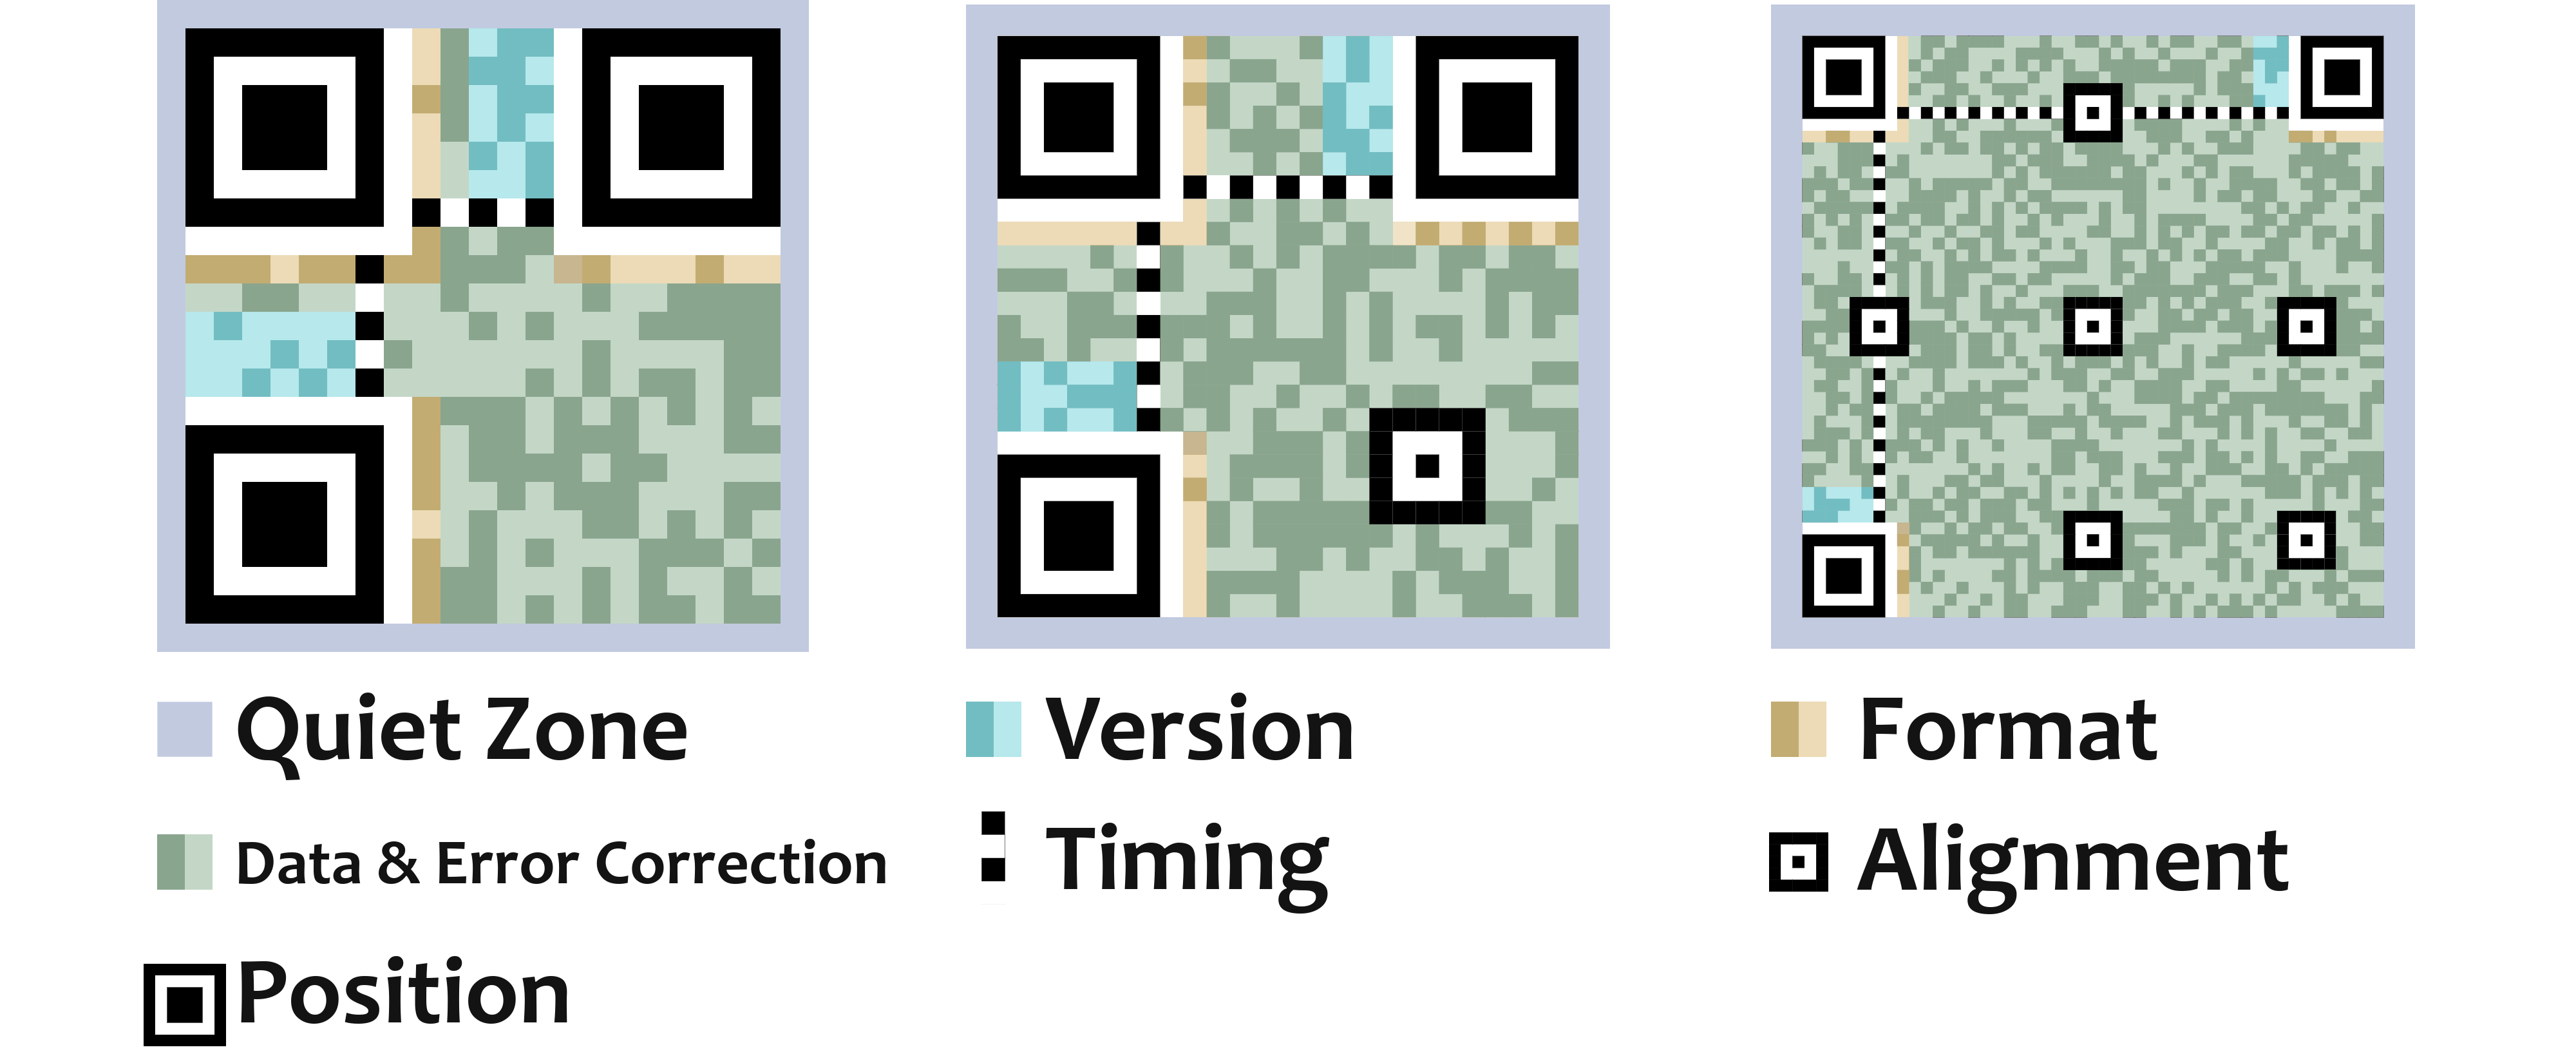
\includegraphics[width=\textwidth]{assets/ch2/QR Codes Figure.png}
	\caption{ These are three QR Codes that store texts. The texts’ lengths get larger going from the left to the right. Notice that the alignment pattern only appears at the bigger QR Codes, and there are multiple ones at the biggest QR Code.}
	\label{QR_code_structure}
\end{figure}

\begin{itemize}
\item \textbf{Quiet Zone:}
This is a white empty area surrounds the QR Code that helps distinguishing it from its surroundings.

\item \textbf{Version Information:} QR Codes have different versions/sizes which specified by these two areas.

\item \textbf{Format Information:}
This part provides details about the error correction level and data mask pattern used.

\item \textbf{Data \& Error Correction:}
This is where both encoded data \& error correction are. data and error correction are stored together enabling the QR code to recover and reconstruct the stored data, even if up to 30\% of the code is damaged or obscured. Data have different types, such as text, URLs, or other. 

\item \textbf{Timing Patterns:}
This part is essential for defining the grid's structure and assists the scanner in establishing the size and coordinate system of the code.

\item \textbf{Alignment Patterns:}
The Alignment Patterns help correct distortion and skewing of the QR code when viewed from different angles. It is especially crucial for larger QR codes that may be prone to bending or misalignment.

\item \textbf{Finder Patterns:}
These patterns assist the scanning device in rapidly locating and orienting the QR code, regardless of its rotation or angle.
\end{itemize}

See \cite{Tiwari2016}, for more information.

\subsection{QR Code Versions and Types}
QR codes come in 40 versions, each representing a different size and data capacity. Version 1 contains 21 × 21 modules, while Version 40 has 177 × 177 modules. As the version number increases, so does the data capacity and the complexity of the code, making it capable of storing more information or supporting higher levels of error correction \cite{Tiwari2016}. 

\begin{figure}[h]
	\centering
	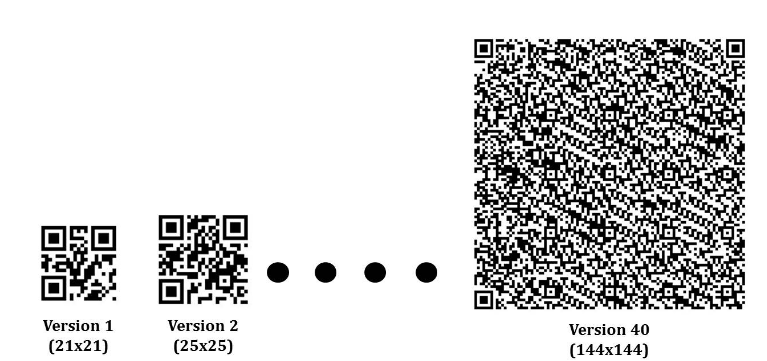
\includegraphics[width=10cm]{assets/ch2/qr_versions}
	\caption{QR codes Versions (adapted from \cite{Tiwari2016}).}
	\label{QR_versions}
\end{figure}


There are also specialized QR code types designed for specific applications:

\begin{itemize}
	\item \textbf{QR Code Model 1 and 2}:
	Model 1 is the original version of the QR code, developed in 1994 by Denso Wave. While model 2 is an improved version of model 1, and it is the one most commonly used today. These models are used for daily basis.
	\item \textbf{Micro QR Code}: Designed to be smaller and simpler, it uses only one Finder Pattern, making it more compact than traditional QR codes. It is often used when space is limited \cite{Tiwari2016}.
	\item \textbf{Logo QR Code}: Allows logos or images to be embedded within the QR code, enhancing the code's visual appeal for marketing or branding purposes \cite{Tiwari2016}.
	\item \textbf{iQR Code}: A flexible matrix-type QR code capable of being printed in various sizes and configurations, from small, high-capacity codes to large codes. It can store more data than standard QR codes and can be inverted or turned into dot patterns for direct part marking \cite{Tiwari2016}.
	\item \textbf{Encrypted QR Code}: Uses encryption techniques to secure the information encoded within, making it suitable for applications requiring data confidentiality \cite{Tiwari2016}.
\end{itemize}

\begin{figure}
	\centering
	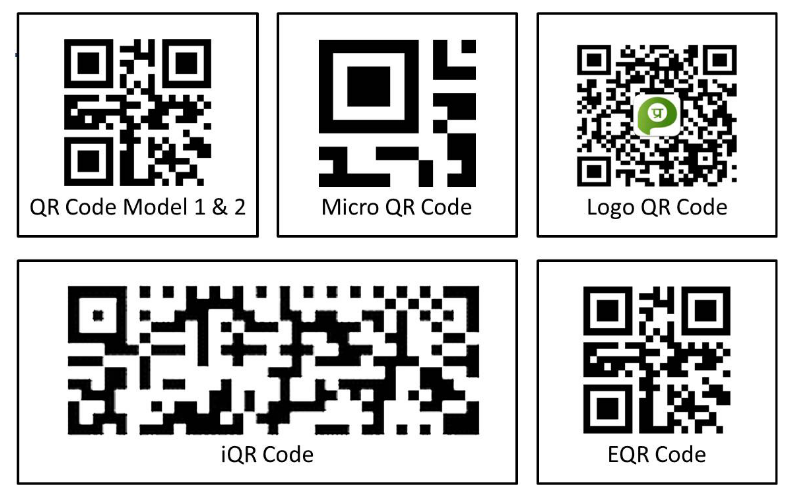
\includegraphics[width=0.7\linewidth]{assets/ch2/qr_codes_type}
	\caption{QR code types (adapted from \cite{Tiwari2016}).}
	\label{qr_code_type}
\end{figure}

\subsection{QR Code Encoding}  
The encoding process for a QR code involves converting data into a matrix of black and white modules. First, the input data is analyzed to determine the appropriate encoding mode, such as numeric, alphanumeric, byte, or Kanji. The data is then transformed into binary code, and error correction is added using Reed-Solomon algorithms, ensuring that the code can still be scanned if partially damaged \cite{Tiwari2016}.

Popular online tools for generating QR codes include:
\begin{itemize}
	\item \textbf{Online Tools}: These free online tools offer simple and fast solutions for both generating and decoding QR codes. QRickit allows users to decode QR codes from uploaded images, while GOQR.me provides various output formats, such as PNG, SVG, and EPS, making it versatile for different use cases \cite{QRCodeMonkey2024}\cite{QRTiger2024}.
	
	
\end{itemize}

For generating QR codes programmatically, popular libraries include:
\begin{itemize}
	\item \textbf{Python - PyQRCode}: A Python library that simplifies QR code creation, allowing output in SVG, PNG, and other formats \cite{PyQRCode2024}.
	\item \textbf{Java - ZXing (Zebra Crossing)}: An open-source library widely used for encoding QR codes in Java and Android applications \cite{ZXing2024}.
	\item \textbf{iOS - Core Image}: iOS provides native QR code generation capabilities via the `CIQRCodeGenerator` filter in the Core Image framework \cite{CoreImage2024}.
\end{itemize}

\subsection{QR Code Decoding}  
\label{qr decode libraries}
Decoding a QR code starts by scanning the Finder Patterns, which allow the scanner to properly align the code. Next, the Format Information is read to apply the correct error correction and mask pattern. Once decoded, the binary data is translated back into the original format (e.g., text, URL) \cite{Tiwari2016}.

Common online tools for decoding QR codes include:
\begin{itemize}
	\item \textbf{Online Tools}: These tools offer versatile QR code decoding solutions across platforms. ZXing is an open-source decoder integrated into Android and web applications, QRickit provides online QR code decoding from uploaded images, and Google Lens allows users to scan and decode QR codes directly via smartphone cameras \cite{ZXing2024, QRickit2024}.
	
\end{itemize}

For decoding programmatically, useful libraries include:
\begin{itemize}
	\item \textbf{Python - Segno}: A versatile Python library for generating and reading both QR and Micro QR codes \cite{Segno2024}.
	\item \textbf{Java - ZXing}: Provides decoding functionality along with encoding, and is widely used for mobile and web apps \cite{ZXing2024}.
	\item \textbf{iOS - AVFoundation}: iOS provides native support for scanning QR codes using the `AVCaptureMetadataOutput` class in the AVFoundation framework \cite{AVFoundation2024}.
	\item \textbf{Google ML Kit}:
	\color{red}temporarily empty...\color{black}
\end{itemize}
 

\section{Indoor Localization}

Indoor localization refers to the process of determining the exact position and orientation of an object or person within indoor environments, where traditional GPS signals are often unreliable. This technology is essential for a wide range of applications, from navigation within large buildings to asset tracking in warehouses.

Various technologies are employed for indoor localization, each with its own strengths and limitations. Wi-Fi, Bluetooth, RFID, and Ultra-Wideband (UWB) are some of the most common methods. While some systems rely on expensive and complex hardware like sensors and Inertial Measurement Units (IMUs), others use more cost-effective solutions such as Bluetooth beacons. The choice of technology often depends on the specific needs of the application, balancing factors such as accuracy, cost, and ease of implementation. For more information, see reference \cite{leitch2023}.

As indoor localization continues to evolve, new techniques and innovative approaches are emerging, including the use of QR codes for precise positioning and tracking. 

\subsection{Indoor Localization with QR Codes}

Indoor localization using QR codes is a method to determine a user’s pose. The system works by strategically placing QR codes around the space—on floors, walls, ceilings, or even hanging panels. Each QR code encodes specific positional information, allowing users to understand their location relative to these codes once they are detected.

\paragraph{Grid Pattern QR codes}

A simple QR-based localization method involves dividing a $n\times m$ meter room into $r$ squares, each with a QR code indicating its exact position. A device, such as a hat with a camera, detects the QR codes as the user moves, determining their location by the square they're in. While this approach provides discrete positional data, it's computationally efficient and useful in contexts like robotics. Although effective for coarse localization, it lacks the precision required for continuous positioning. This approach is used in the solution proposed by \cite{zhang2015}.

\begin{figure}[h] % [h] forces the figure to be placed exactly here in the text
	\centering
	\includegraphics[width=5cm]{example-image-A}
	\caption{Grid Patter Illustration}
	\label{grid_pattern_illustration}
\end{figure}



\paragraph{Pose Estimation with QR codes}

Another approach of indoor localization involves calculating the relative position and orientation (pose) of the QR code in relation to the camera. After detecting a QR code, the camera determines its position and orientation relative to itself, and by combining this information with the known global position of the QR code, the system can estimate the user’s precise, continuous position within the space. Although this method offers significantly higher positional accuracy, it requires more computational resources, as it involves additional steps such as camera calibration to determine intrinsic parameters. This added complexity makes it more resource-intensive compared to grid-based localization, but it delivers continuous localization with greater precision. \textcolor{red} {Cite the papar that use this approach}

\begin{figure}[h] % [h] forces the figure to be placed exactly here in the text
	\centering
	\includegraphics[width=5cm]{example-image-A}
	\caption{Grid Patter Illustration}
	\label{pose_estimation_illustration}
\end{figure}


In a well-designed setup, the system's effectiveness remains high, irrespective of the QR codes’ locations. By tailoring the placement and setup of QR codes to suit the environment, the system can deliver robust indoor localization, whether it prioritizes simplicity or precision.
\section{Objects Detection}


\section{Customizable Guidance}


\section{Related Work}

In localization research, artificial landmarks have been widely utilized due to the challenges associated with detecting and building systems based on natural landmarks. Among artificial landmarks, QR codes have garnered significant attention because of their ease of creation, low implementation costs, and the substantial amount of information they can encode.

The work of Zhang et al. \cite{zhang2015} presents an approach for indoor mobile robot localization using QR codes arranged in a grid pattern on the ceiling. The system uses an industrial camera mounted on top of the robot, facing upward to detect these QR codes. The camera captures images of the QR codes, and a recognition algorithm processes the codes' position and orientation within the image. By leveraging the coordinates of each QR code and applying camera calibration data, the robot can accurately determine its position. This setup enables real-time, precise localization, which is crucial for efficient navigation in structured indoor environments.

Kim et al. \cite{kim2021} introduce a vision-based indoor positioning system that employs QR codes and a smartphone camera to accurately determine a user's indoor location. In this system, QR codes are placed at predefined locations and detected by the smartphone camera. The two-dimensional coordinates from the QR codes are converted into three-dimensional spatial coordinates using camera calibration techniques. By forming a quadrilateral shape from reference symbols on the QR codes, the system calculates the center of gravity to determine the user's position and orientation. Experiments demonstrated an average localization error of less than one meter, highlighting the system's high accuracy.

Lee et al. \cite{lee2015} propose a cost-effective indoor localization method for mobile robots, using QR codes as artificial landmarks. QR codes are strategically placed on the ceiling, and a smartphone mounted on the robot detects these codes to determine the robot’s position and heading direction. The positions of the QR codes are pre-stored in a database, enabling the robot to compute its real-world coordinates by processing image data captured by the smartphone's camera. The system has been experimentally validated, showing localization errors ranging from 3.2 cm to 6.55 cm, confirming its accuracy.

\textcolor{blue}{We should mention as a conclusion of this section how our solution will differ from them whether by accuracy, multiple tech integration, targeted audience, real world validation method, etc.}


% ========= BEGIN: CHAPTER-3 ======== %
\chapter{Methodology}
\newpage
\section{System Architecture Overview}

This section provides an overview of the architecture of our indoor navigation system, designed to assist visually impaired users with real-time, context-aware guidance within indoor environments. The system leverages a combination of mobile technology, backend services, and sensory input devices to deliver seamless and accessible navigation. Below, we present the key components, data flow, technology stack, and a system diagram to illustrate the complete structure of the system.

\subsection{High-Level View of Components}

The system is composed of several interacting components:

\begin{itemize}
	\item \textbf{Mobile Application}: The main user interface for visually impaired users. This application handles QR code scanning, voice command processing, navigation feedback (both audio and vibration), and integration with external devices (e.g., camera, microphone).
	\item \textbf{QR Code Scanner and Object Detection}: The mobile app uses a camera sensor connected to an ESP32 microcontroller to scan QR codes and detect key objects, such as trashcans and chairs, within the environment. YOLOv10 is employed for efficient object detection, while Google’s ML Kit is used for QR code scanning.
	\item \textbf{Navigation and Guidance System}: This module within the mobile application provides real-time navigation assistance based on the user’s location, direction, and desired destination. It uses data from QR codes and object detection to inform users about nearby obstacles and paths.
	\item \textbf{Backend and Database}: A cloud-based backend server and database store user and navigation data, such as QR code global positions, custom instructions, and map layouts. The server processes requests for location-specific information and delivers relevant navigation instructions to the app.
	\item \textbf{I/O Devices and ESP32 Microcontroller}: An ESP32 microcontroller manages additional components, including a camera module for QR code scanning, an ultrasonic sensor for obstacle detection, and a speaker for audio output. The ESP32 also transmits audio and tactile feedback to guide users.
\end{itemize}

\subsection{Data Flow}

The system’s data flow is designed for efficient and seamless interactions across components. Below is an outline of the primary data flow:

\begin{enumerate}
	\item \textbf{QR Code Scanning and Localization}: The camera captures a frame containing a QR code, which the app decodes using ML Kit. The app then retrieves the global position of the QR code from the backend, which provides a reference point for the user’s current location.
	\item \textbf{Navigation Instruction Retrieval}: After the QR code is decoded, the mobile app queries the backend for location-specific instructions, which are returned in real-time and provided to the user as audio guidance.
	\item \textbf{Voice Command Processing}: Users can interact with the navigation system via voice commands. The app processes these commands locally and may query the backend if needed for contextual information (e.g., “Guide me to the nearest exit”).
	\item \textbf{Object Detection and Proximity Alerts}: The ESP32 detects nearby obstacles using the ultrasonic sensor and sends alerts to the mobile app, which provides vibration feedback to notify users.
	\item \textbf{Customizable Guidance Updates}: When users reach specific points (QR codes or predefined milestones), the app provides updated instructions tailored to the current context, based on backend data.
\end{enumerate}

\subsection{Technology Stack}

The following tools and technologies were selected for each component of the system:

\begin{itemize}
	\item \textbf{Mobile Application Development}: Developed using Kotlin.
	\item \textbf{QR Code Scanning and Object Detection}: Google ML Kit is used for QR code detection and decoding, while YOLOv10 (converted to TensorFlow Lite) performs real-time object detection.
	\item \textbf{Navigation and Guidance Logic}: Implemented with OpenCV for pose estimation and CameraX for real-time camera access.
	\item \textbf{Backend and Database}: SQLite3 for lightweight database, FastAPI for quick and easy to deploy API, Python for other services such as QR code generation. 
	\item \textbf{ESP32 Microcontroller and Sensors}: The ESP32 is programmed to control the camera, ultrasonic sensor, and speaker, utilizing TensorFlow Lite for lightweight operations on embedded devices.
\end{itemize}


\section{Localization System}
The basic idea behind our localization system implementation is to capture a frame at real time by a camera, then detect and decode the QR code in it. After that, we will be able to restore the QR code's global position from the server using the decoded data, \color{blue}which is described at...(write where) \color{black}. Now, we only need to calculate the camera's position relative to the QR code, and then add the result together with the QR code's global position as follows:
\[ user\_global\_position = QR\_global\_position +  camera\_relative\_position\]
This is the pose estimation approach which is mentioned previously at section \ref{Pose Estimation with QR Codes BG}.

As we just mentioned, the QR code's global position is stored at a server so there is nothing to calculate here, but this is not the case of the camera's relative position. The process of calculating the later is somewhat complicated and not short, and there are several things that need to be calculated first, such as the QR code corners locations at the image frame, camera matrix, and the camera distortion coefficients. There are multiple libraries for localization purposes as we mentioned previously at \ref{localization libraries BG}, and we choose OpenCV due to its Android devices support, ease of use, simple API, and performance.

Everything related to the localization will be running at a separate thread from the main thread. This enables the System to perform other tasks simultaneously and independently.

\subsection{Camera Calibration}
We mentioned \color{blue}at...(write where) \color{black} that users can chose the camera they want to use from the settings after connecting it to the phone. This approach rise the need of calibration system that users can use since the cameras' parameters are distinct and not known. Each camera need to be calibrated at least once at the first time. Then the camera parameters will be stored at the phone storage for reusing in the future. At first, users need to specify the number of rows and columns at the pattern and the width/height of each square in real world units. Then they need to take multiple photos to the pattern at different angles and distances and start the calibration process. After this point, everything else will be done automatically without the need of the users actions no more. 

The camera calibration system's implementation is the same as what was mentioned previously at section \ref{Camera Calibration Background}. First the program will iterate through each photo trying to estimate their inner corners points locations using the following OpenCV function:
\begin{lstlisting}[language=Java]
boolean findChessboardCorners(
	Mat image,
	Size patternSize,
	MatOfPoint2f corners
)
\end{lstlisting}

\subparagraph{Params:}

\begin{itemize}
	\item \textbf{image:}
	The current photo of the pattern.
	\item \textbf{patternSize:}
	Number of inner corners per a chessboard row and column.
	\item \textbf{corners:}
	Output array of detected corners.
\end{itemize}

After that, we used the OpenCV function cornerSubPix to refine the detected points. Finally, we used the following OpenCV function for calibration:
\begin{lstlisting}[language=Java]
double calibrateCamera(
	List<Mat> objectPoints,
	List<Mat> imagePoints, 
	Size imageSize, 
	Mat cameraMatrix, 
	Mat distCoeffs, 
	List<Mat> rvecs, 
	List<Mat> tvecs
)
\end{lstlisting}

\subparagraph{Params:}

\begin{itemize}
	\item \textbf{objectPoints:}
	List of real world inner points locations for each image.
	\item \textbf{imagePoints:}
	List of estimated inner points locations for each image.
	\item \textbf{imageSize:}
	Size of the calibrated pattern photo.
	\item \textbf{cameraMatrix:}
	Output matrix for the camera intrinsic values.
	\item \textbf{distCoeffs:}
	Output matrix for the camera distortion coefficients.
	\item \textbf{rvecs:}
	Output list contains the rotation of the calibration patterns for each image.
	\item \textbf{tvecs:}
	Output list contains the translation of the calibration patterns for each image.
\end{itemize}

\subsection{Camera's Relative Pose}
The first step is to capture frames using a camera at real time. We used cameraX to do so since it is the best for Android devices as we mentioned at \ref{localization libraries BG}. Then, each captured frame will be passed to a function for QR code detecting, decoding, and pose estimation, so finally we can calculate camera's relative position. For QR code detecting, there are bunch of useful libraries we can for QR code detecting and decoding as we mentioned previously at \ref{qr decode libraries}. We choose Google's ML kit due to its simplicity and good performance. After successfully detecting the QR code, Google's ML kit will calculate the QR code corners locations for us.

Finally, we use OpenCV's solvePnP to calculate the QR pose function as follow:

\begin{lstlisting}[language=Java]
boolean solvePnP(
	MatOfPoint3f objectPoints, 
	MatOfPoint2f imagePoints, 
	Mat cameraMatrix, 
	MatOfDouble distCoeffs, 
	Mat rvec, 
	Mat tvec
)
\end{lstlisting}

\subparagraph{Params:}

\begin{itemize}
	\item \textbf{objectPoints:}
	The QR code's four corners locations relative to its center in real world units, such as cm, mm, etc.
	\item \textbf{imagePoints:}
	The locations of the QR code's corners inside the captured frame in pixels.
	
	\item \textbf{cameraMatrix \& distCoeffs:}
	These two are crucial for calculating the QR code's pose since they represent the intrinsic values of a camera and its distortion coefficients.
	
	\item \textbf{rvec \& tvec:}
	These are output vectors for the code's rotation(rvec) and translation(tvec) relative to the camera.
\end{itemize}
imagePoints is calculated after successfully detecting the QR code by Google's ML kit.

Now we got the QR code's translation vector relative to the camera, we just multiply it with -1 to get the camera translation relative to the QR code.

% ========= BEGIN: CHAPTER-4 ======== %
\chapter{Results and Discussion}
\newpage
\section{Results}



% ========= BEGIN: CHAPTER-5 ======== %
\chapter{Conclusion and Future Work}
\newpage
\section{Conclusion and Future Work}

The project concludes by summarizing the findings and suggesting future work.



%Figure \ref{fig:future_work} highlights potential areas for future research and development.




\newpage
\addcontentsline{toc}{chapter}{References}
\renewcommand{\bibname}{References}

\begin{thebibliography}{9}
	\bibitem{Fiducial2021}
	Michail K., Brennan C., Sabrina C., Anand A., Camden W., \& Nikolaos
	V. (2021). Fiducial Markers for Pose Estimation. Journal of Intelligent \&
	Robotic Systems (2021) 101:71.
	https://link.springer.com/article/10.1007/s10846-020-01307-9
		
	\bibitem{Tiwari2016} Tiwari, V., "QR Code Technology and Its Applications," International Journal of Advanced Research in Computer Science and Software Engineering, vol. 6, no. 4, pp. 123-127, 2016.
	
	\bibitem{AndroidWebsite}
	Android, "Official Android Website," Available: \url{https://www.android.com/}.
	
	
	\bibitem{EspressifModules}
	Espressif Systems, "ESP Modules," Available: \url{https://www.espressif.com/en/products/modules}.
	
	\bibitem{GoogleTalkBack}
	Google Accessibility, "Use TalkBack on Android Devices," Available: \url{https://support.google.com/accessibility/android/topic/10601571?hl=en&ref_topic=3529932}.
	
	\bibitem{SingleCamera3D}
	E. Chian, "A Single Camera 3D Functions," Medium, Available: \url{https://eugene-chian.medium.com/a-single-camera-3d-functions-fdec7ffa9a83}.
	
	
	
	
	\bibitem{zhang2015}
	H. Zhang, C. Zhang, W. Yang and C. -Y. Chen, "Localization and navigation using QR code for mobile robot in indoor environment," 2015 IEEE International Conference on Robotics and Biomimetics (ROBIO), Zhuhai, China, 2015, pp. 2501-2506, doi: 10.1109/ROBIO.2015.7419715.
	
	\bibitem{ahmetovic2016}
	D. Ahmetovic, C. Gleason, C. Ruan, K. M. Kitani, H. Takagi and C. Asakawa, "NavCog: a navigational cognitive assistant for the blind," *Proceedings of the 18th International Conference on Human-Computer Interaction with Mobile Devices and Services*, Florence, Italy, 2016, pp. 90-99, doi: 10.1145/2935334.2935361.
	
	\bibitem{ibm2024}
	IBM, "What Is an API (Application Programming Interface)?," *IBM Topics*, 2024. [Online]. Available: https://www.ibm.com/topics/api. [Accessed: 28-Oct-2024].
	
	\bibitem{visual-paradigm}
	Visual Paradigm, "What Is Entity Relationship Diagram?," *Visual Paradigm*, 2024. [Online]. Available: https://www.visual-paradigm.com/guide/data-modeling/what-is-entity-relationship-diagram/. [Accessed: 28-Oct-2024].
	

	\bibitem{Lucag2017}
	Luca C., Gionata C., Francesco F., Alessandro F., Gianluca I., Andrea M. Federica V. (2017). A QR-code Localization System for Mobile Robots: Application to Smart Wheelchairs.
	https://ieeexplore.ieee.org/document/8098667
	
	\bibitem{VybronicsVC0820B006F}
	Vybronics, "VC0820B006F Coin Vibration Motor Datasheet," 
	Available: \url{https://www.vybronics.com/wp-content/uploads/datasheet-files/Vybronics-VC0820B006F-datasheet.pdf}.
	
	
	\bibitem{HCSR04Datasheet}
	SparkFun Electronics, "Ultrasonic Ranging Module HC-SR04 Datasheet," 
	Available: \url{https://cdn.sparkfun.com/datasheets/Sensors/Proximity/HCSR04.pdf}.
	
	
	\bibitem{kim2021}
	J.-I. Kim, H.-S. Gang, J.-Y. Pyun, and G.-R. Kwon, "Implementation of QR Code Recognition Technology Using Smartphone Camera for Indoor Positioning," Energies, vol. 14, no. 10, p. 2759, 2021, doi: 10.3390/EN14102759.
	
	\bibitem{lee2015}
	S. -J. Lee, G. Tewolde, J. Lim and J. Kwon, "QR-code based Localization for Indoor Mobile Robot with validation using a 3D optical tracking instrument," 2015 IEEE International Conference on Advanced Intelligent Mechatronics (AIM), Busan, Korea (South), 2015, pp. 965-970, doi: 10.1109/AIM.2015.7222664.
	
	\bibitem{kalaitzakis2021} 
	M. Kalaitzakis, B. Cain, S. Carroll, A. Ambrosi, C. Whitehead, and N. Vitzilaios, "Fiducial Markers for Pose Estimation: Overview, Applications, and Experimental Comparison of the ARTag, AprilTag, ArUco, and STag Markers," Journal of Intelligent \& Robotic Systems, vol. 101, no. 71, pp. 1-26, 2021, doi: 10.1007/s10846-020-01307-9.
	
	\bibitem{Aqeel Anwar}
	Aqeel Anwar, "What are Intrinsic and Extrinsic Camera Parameters in Computer Vision?", A detailed explanation of intrinsic and extrinsic camera parameters with the help of visualizations.
	https://towardsdatascience.com/what-are-intrinsic-and-extrinsic-camera-parameters-in-computer-vision-7071b72fb8ec
	
	\bibitem{kuribayashi2023}
	M. Kuribayashi, T. Ishihara, D. Sato, J. Vongkulbhisal, K. Ram, S. Kayukawa, H. Takagi, S. Morishima and C. Asakawa, "PathFinder: Designing a Map-less Navigation System for Blind People in Unfamiliar Buildings," *Proceedings of the 2023 CHI Conference on Human Factors in Computing Systems (CHI '23)*, New York, NY, USA, 2023, Article 41, pp. 1–16, doi: 10.1145/3544548.3580687.
	
	\bibitem{fraga2022}
	A. L. Fraga, X. Yu, W.-J. Yi, and J. Saniie, "Indoor Navigation System for Visually Impaired People using Computer Vision," *2022 IEEE International Conference on Electro Information Technology (eIT)*, Grand Forks, ND, USA, 2022, pp. 257-260, doi: 10.1109/eIT53694.2022.9800294.
	
	\bibitem{whichCameraLibToUse}
	https://developer.android.com/media/camera/choose-camera-library
	
	\bibitem{Tiwari2016}
	S. Tiwari, "An Introduction to QR Code Technology," 2016 International Conference on Information Technology (ICIT), Bhubaneswar, India, pp. 39-44, 2016, doi: 10.1109/ICIT.2016.021.
	
	\bibitem{leitch2023} S.G. Leitch, Q.Z. Ahmed, W.B. Abbas, M. Hafeez, P.I. Laziridis, P. Sureephong, and T. Alade, "On Indoor Localization Using WiFi, BLE, UWB, and IMU Technologies," Sensors, vol. 23, no. 20, pp. 8598, 2023, doi: 10.3390/s23208598.
	
	\bibitem{QRCodeMonkey2024} "QRCode Monkey - Free QR Code Generator," QRCode Monkey, Available: \url{https://www.qrcode-monkey.com}.
	
	\bibitem{QRTiger2024} "QR TIGER - Free QR Code Generator," QR Tiger, Available: \url{https://www.qrcode-tiger.com}.
	
	
	\bibitem{PyQRCode2024} "PyQRCode Documentation," PyQRCode, Available: \url{https://pyqrcode.readthedocs.io}.

	\bibitem{ZXing2024} "ZXing Decoder," ZXing Project, Available: \url{https://github.com/zxing/zxing}.

	\bibitem{CoreImage2024} "Core Image Framework," Apple Developer Documentation, Available: \url{https://developer.apple.com/documentation/coreimage}.

	\bibitem{Segno2024} "Segno - Python QR Code Generator," Segno Documentation, Available: \url{https://segno.readthedocs.io}.

	\bibitem{AVFoundation2024} "AVFoundation Framework," Apple Developer Documentation, Available: \url{https://developer.apple.com/documentation/avfoundation}.

	\bibitem{SebastianLague_AStar}
	https://www.youtube.com/watch?v=-L-WgKMFuhE\&list=
	PLFt AvWsXl0cq5Umv3pMC9SPnKjfp9eGW

	\bibitem{QRickit2024} "QRickit QR Code Decoder," QRickit, Available: \url{https://qrickit.com}.
	
	\bibitem{OV5640}
	OmniVision Technologies. (2008). 5-Megapixel SOC Camera Module. 
	https://cdn.sparkfun.com/datasheets/Sensors/LightImaging/OV5640\_datasheet.pdf
	
	\bibitem{OV7670}
	OmniVision Technologies. (2006). OV7670 Camera Module Datasheet. 
	https://web.mit.edu/6.111/www/f2016/tools/OV7670\_2006.pdf
	
	\bibitem{OV2640}
	OmniVision Technologies. (2016). OV2640 Camera Module Datasheet. 
	https://www.uctronics.com/download/OV2640\_DS.pdf
	
	
	
\end{thebibliography}

\newpage
\fancyhead[L]{\text{Appendix \thechapter{}}}
\addcontentsline{toc}{chapter}{Appendices}
\appendix % Switch to appendices mode

\chapter{}
\section{Sample Data Tables}

Here we provide some example data tables that might be relevant for the study.

\begin{table}[h!]
\centering
\caption{Example Data Table}
\begin{tabular}{|l|c|r|}
\hline
\textbf{Item} & \textbf{Quantity} & \textbf{Price} \\
\hline
Item 1 & 10 & \$100 \\
Item 2 & 20 & \$200 \\
Item 3 & 30 & \$300 \\
\hline
\end{tabular}
\end{table}

\section{Sample Figures}

Below is an example figure for demonstration purposes.



\chapter{}
\section{Additional Information}

This appendix contains additional information relevant to the study, including supplementary materials and further explanations.

\section{Supplementary Materials}

Here you might include additional data or documents that support your research.

\section{Further Explanations}

This section provides further explanations on specific topics covered in the main document. For example, you might elaborate on methodologies or provide additional insights into the analysis.

\end{document}


\end{document}
